\documentclass{beamer}
\usepackage[orientation=portrait,size=a0,scale=1.52,debug]{beamerposter}
\mode<presentation>{\usetheme{ZH}}
\usepackage[utf8]{inputenc}
\usepackage[german, english]{babel} % required for rendering German special characters
\usepackage{siunitx} %pretty measurement unit rendering
\usepackage{hyperref} %enable hyperlink for urls
\usepackage{ragged2e}
\usepackage[font=scriptsize,justification=justified]{caption}
\usepackage{array,booktabs,tabularx}
\usepackage{color}
\usepackage{centernot}

\newcolumntype{Z}{>{\centering\arraybackslash}X} % centered tabularx columns
\sisetup{per=frac,fraction=sfrac}

\title{\huge Pairwise Webpage Coreference Classification using Distant Supervision}
\author{S. Shivashankar, Timothy Baldwin, Julian Brooke, Trevor Cohn}
\institute[The University of Melbourne]{Computing and Information Systems, The University of Melbourne, Australia}
\date{April 5, 2017}

% edit this depending on how tall your header is. We should make this scaling automatic :-/
\newlength{\columnheight}
\setlength{\columnheight}{104cm}

\newcommand{\query}[1]{\texttt{#1}\xspace}
\newcommand{\ex}[1]{\textit{#1}\xspace}
\newcommand{\tabref}[1]{Table~\ref{#1}\xspace}
\newcommand{\secref}[2][]{Section#1~\ref{#2}\xspace}

\begin{document}
\begin{frame}
\begin{columns}
	\begin{column}{.5\textwidth}
		\begin{beamercolorbox}[center]{postercolumn}
			\begin{minipage}{.98\textwidth}  % tweaks the width, makes a new \textwidth
				\parbox[t][\columnheight]{\textwidth}{ % must be some better way to set the the height, width and textwidth simultaneously
					\begin{myblock}{Introduction}
						\textbf{A person or other entity is often associated with multiple URL endpoints on the web}
						\vspace{0.5em}
			               \begin{itemize}
			                \item { \color{gray} \tt Barack Obama} $\Leftrightarrow$ {\color{blue} \small \url{barackobama.com/}} and {\color{blue} \small \url{en.wikipedia.org/wiki/Barack_Obama}}
					\item { \color{gray} \tt Donald Trump} $\centernot\Leftrightarrow$ {\color{blue} \small \url{twitter.com/realDonaldTrump}} and {\color{blue}  \small \url{instagram.com/ivankatrump}}
			                \end{itemize}
	              {\color{cyan} Motivates the task of  \textbf{webpage coreference classification} for a given entity!}
    				\end{myblock}\vfill
					\begin{myblock}{Problem Setup}
						\vspace{0.5em}
	 \begin{itemize}
	\item We assume access to web KBs based on automatic crawling
	\begin{itemize}
	 \item social networks (e.g. {\color{blue} \url{facebook.com/*})}, news aggregation endpoints (e.g. {\color{blue} \url{nytimes.com/topic/person/*}}) and organisation directories (e.g.  {\color{blue} \url{gtlaw.com/People/*}})
	\end{itemize}     	
\item  Given a training dataset $D$ with pairs of web URLs 
         \begin{itemize}
\item Initially all the pairs are unlabeled ($D_{u} \leftarrow D$, $D_{p}, D_{n} = \phi$)
\item Learn a model \begin{small} $\quad f(\phi(U_{i}, U_{j})) \to y$ \end{small}, for URL pair $U_{i}$ and $U_{j}$
\item Target $y \in \{0,1\}$ 
	\end{itemize}     		
	\end{itemize}     		
    				\end{myblock}\vfill
					\begin{myblock}{Distant Supervision}
			%\begin{figure}
			%				\begin{minipage}{0.94\textwidth}
			%					\centering\includegraphics[height=0.7\textwidth, width=0.7\textwidth, keepaspectratio]{img/DS2.png}
			%				\end{minipage}
			%			\end{figure}

\vspace{0.5em}

              \begin{itemize}
		\item  We obtain positive examples using web-search-based distant supervision
		\item  Search query {\color{gray} \tt George Clinton AND P-Funk} fetches {\small \color{blue} \url{en.wikipedia.org/wiki/George_Clinton_(musician)}}
		\begin{itemize}
		\item But not {\small \color{blue} \url{biography.com/people/george-clinton-537674}}
     \end{itemize}     
		\item  We build a positive and unlabelled (PU) learning model
     \end{itemize}     
						\vspace{0.5em}
			
					\end{myblock}\vfill
					\begin{myblock}{Proposed Approach}

              \begin{itemize}
		\item  We generate queries for URL pairs that share same entity name
		\item  Employ a label propagation technique to expand the set of positive examples
     \end{itemize}     
						\vspace{0.5em}
						\begin{figure}
							\begin{minipage}{0.94\textwidth}
								\centering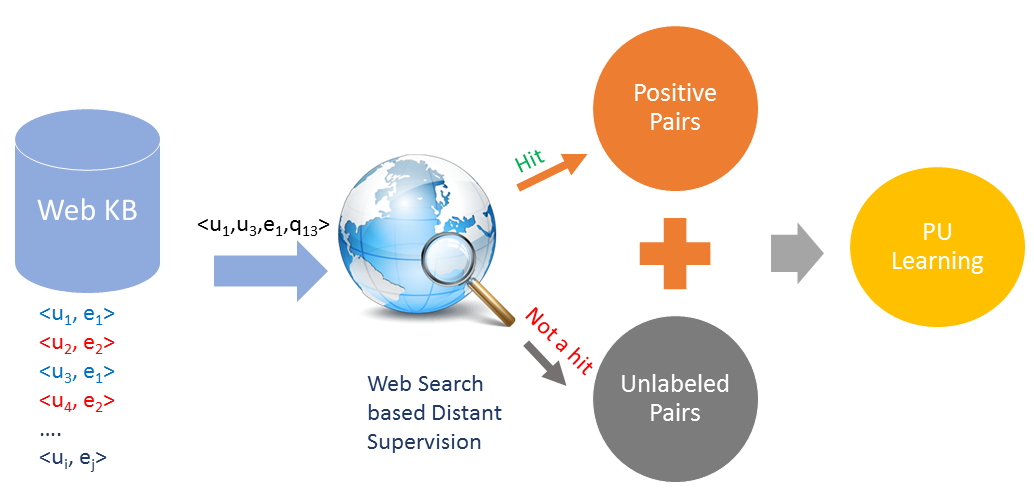
\includegraphics[height=0.7\textwidth, width=1\textwidth, keepaspectratio]{img/FlowWWW1.png}
							\end{minipage}
						\vspace{0.5em}

						\end{figure}
             \begin{itemize}
		\item Any binary classifier can be trained on the expanded labeled set 
     \end{itemize}     
					\end{myblock}\vfill

         \begin{block}{Query Generation}
\begin{itemize}
\item We construct web search queries for distant supervision as follows:
\begin{itemize}
\item \textbf{$Q_i$:} Using the target entity name and context information from $U_{i}$
\item \textbf{$Q_j$:} Similar to the above, we generate context information from  $U_{j}$.
\end{itemize}
\item E.g., for URL pairs: {\color{blue} \small \url{www.imperial.ac.uk/people/f.allen}} and {\color{blue} \small \url{www.linkedin.com/in/franklin-allen-0557906}}
a query constructed is {\color{cyan} \tt \small {"Franklin Allen Brevan Howard Centre"}}
\end{itemize}
\vspace{0.5em}
\end{block} \vfill
		}\end{minipage}\end{beamercolorbox}
	\end{column}
	\begin{column}{.5\textwidth}
		\begin{beamercolorbox}[center]{postercolumn}
			\begin{minipage}{.98\textwidth} % tweaks the width, makes a new \textwidth
				\parbox[t][\columnheight]{\textwidth}{ % must be some better way to set the the height, width and textwidth simultaneously



\begin{block}{Label Propagation using Distant Supervision}
\begin{itemize}
\item For each query in $Q_i$, we check to see if $U_{j}$ is present in the top-$K$ search results $S_{ij}$
	\vspace{0.5em}
\item Conversely if $U_i$ is present in the top-$K$ results, $S_{ji}$ for each query in $Q_j$
	\vspace{0.7em}
\begin{itemize}
\item $[ \, \exists  q \in Q_i,  \quad \exists S_{ji} \mid U_j \in S_{ji} \lor \exists q \in Q_j,  \quad \exists S_{ij} \mid U_i \in S_{ij} ] \, \implies \hat{y_{ij}}=1$
	\vspace{0.7em}
\item $D_{p} \gets D[\hat{y_{ij}}=1]$, $D_{u} \gets D_{u} \setminus D[\hat{y_{ij}}=1]$.
\end{itemize}
\end{itemize}
\vspace{0.5em}

\item \textbf{Expand Positive Labeled Set:}
\begin{itemize}
\item Step 1: Randomly select $N$ instances from $D_{p}$, and hold them out in $S_{p}$.
	\vspace{0.5em}
\item Step 2: Train a binary classifier $\theta$, taking $D'_{p} = D_p \setminus S_p$ as positive instances and $D_{u}$ as negative instances. 
	\vspace{0.5em}
\item Step 3: \mbox{$\mu_{p} = \frac{1}{|S_{p}|}\sum_{i:S_{p}} p(x_{i}=1 | \theta)$,} (using Platt scaling)
	\vspace{0.5em}
\begin{itemize}
\item $D_p^* = {x_u \in D_u: p(x_{u}=1) > \mu_{p}}$.
	\vspace{0.5em}
\item $D_{p} \leftarrow D_{p} \cup D_{p}^*$, $D_{n} \leftarrow D_{u} \setminus D_{p}^*$
\vfill
\end{itemize}
              \end{itemize}
\vspace{0.5em}
            \end{block}
            \vfill
					
	\begin{myblock}{Datasets}
        \begin{itemize}
        \item SemEval-2007 WePS development set 
	\begin{itemize}
		\item Balanced 1000 end-point URL-pairs dataset from webpages for 49 people. 
	%	\item Use a random 70/30 split for training and testing
	\end{itemize}	
	\vspace{0.5em}
	\item ALTA-2016 shared task dataset
	 	\begin{itemize}
		\item Balanced 400 end-point URL-pairs dataset that can refer to any entity 
	%	\item We used 300 pairs for training, and the contest's heldout set of 100 pairs for testing. 
	      \end{itemize}
          \end{itemize}
        \end{myblock} \vfill

%\vspace{0.5em}
  \begin{block}{Feature Representation}

% \item Feature Representation
	      \begin{itemize}
		\item Structural features such as document length difference, URL path length difference
	\vspace{0.5em}
		\item Semantic features such as unigram cosine similarity, cosine similarity over an average word-level word2vec representation, machine translation scores (BLEU, METEOR, TER)
		\end{itemize}	
    \end{block}
\vfill

                        \begin{block}{Experimental Results}
    \begin{itemize}
              \item Benchmark Approaches
                \begin{itemize}
                \item {\color{blue} Biased SVM (BSVM)} with costs for positive and negative classes
                \item {\color{brown} Spy-SVM} (B. Liu et. al., ICML 2002)
		\item {\color{cyan} SPUL} (C. Elkan et. al., KDD 2008)
                \item {\color{gray}Hierarchical Clustering (HC)} - Unsupervised Approach
              \end{itemize}
	      \item Proposed Approach
                \begin{itemize}
\item {\color{violet} DP-SVM} (Linear Kernel SVM built using propagated distant labels)
              \end{itemize}
     \end{itemize}
              \begin{figure}
                \footnotesize
                \centering

        \begin{figure}
							\begin{minipage}{1.22\textwidth}
								\centering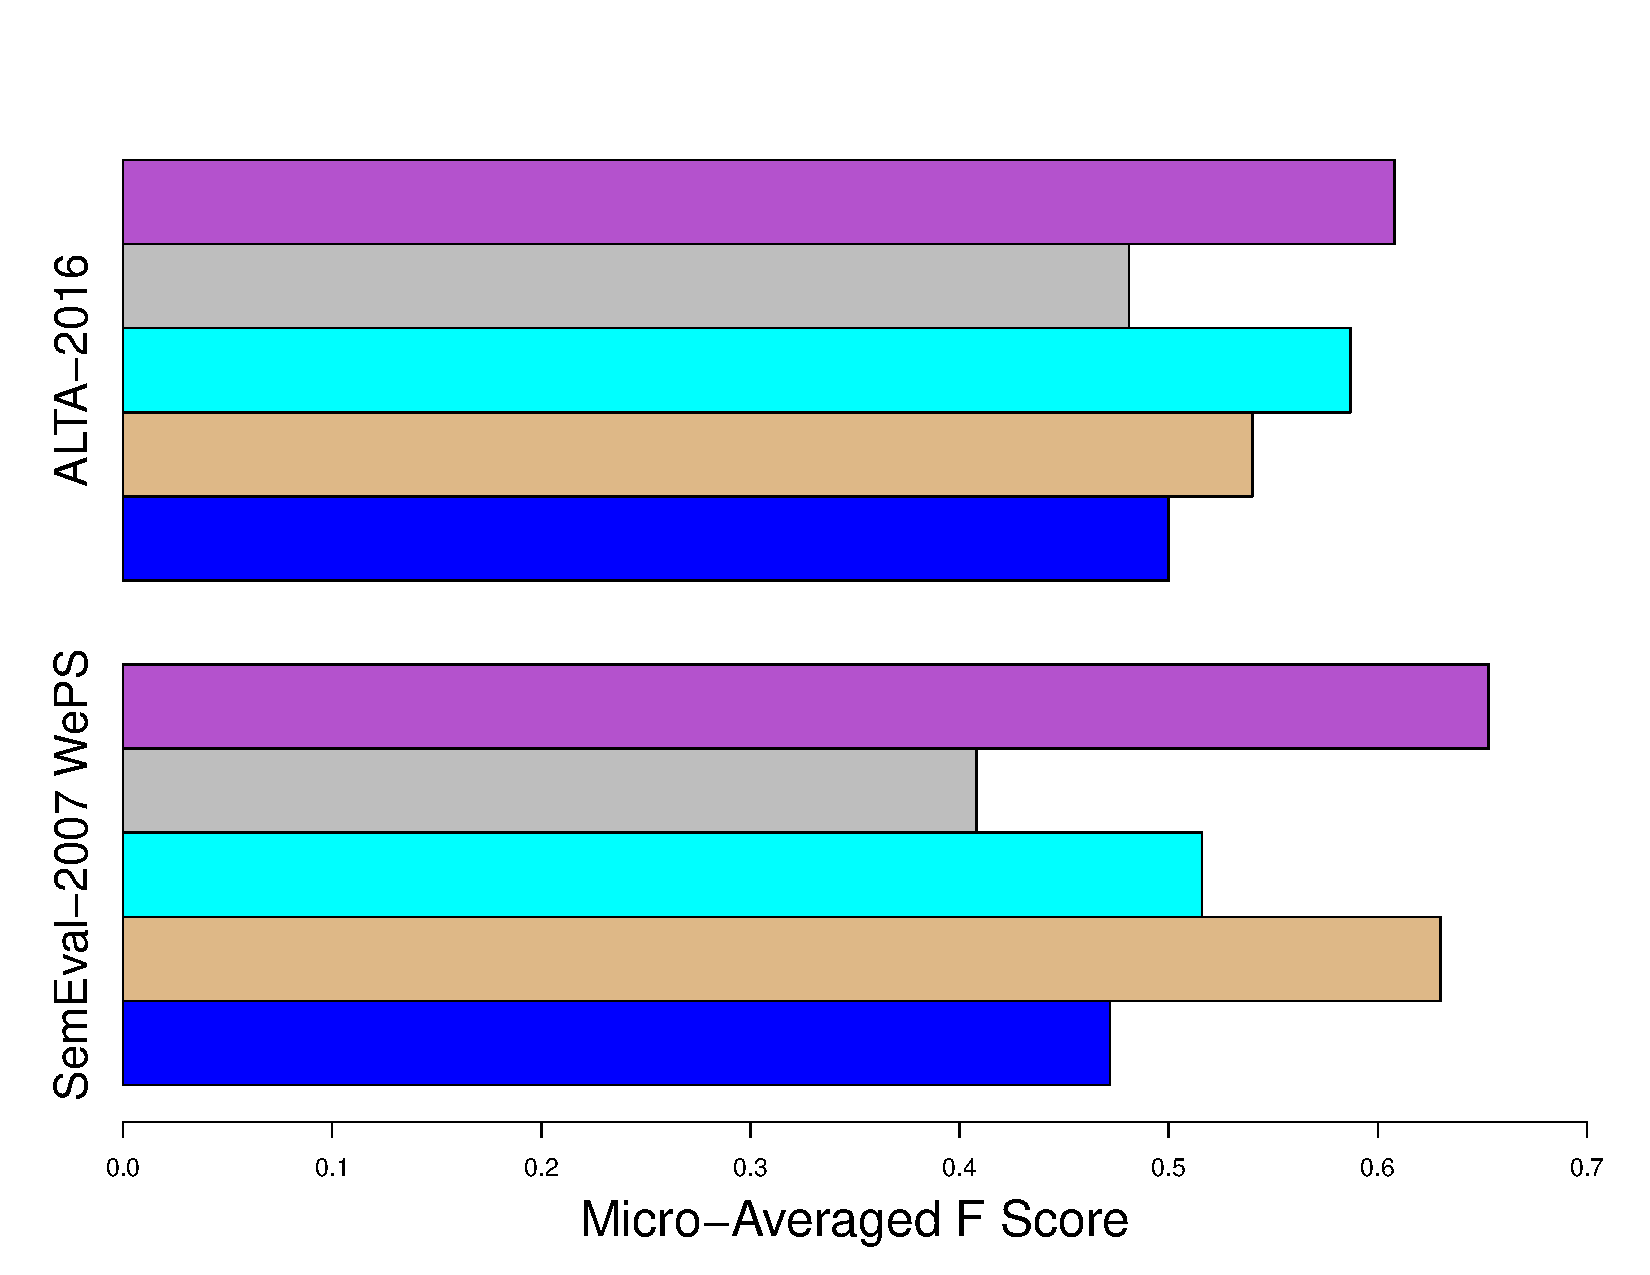
\includegraphics[height=0.4\textwidth,width=1.25\textwidth,keepaspectratio]{img/ResultsWWW8.pdf}
							\end{minipage}
						\end{figure}
%\begin{table}[t]
%  \centering
%\begin{small}
% \begin{tabular}{lcccccc}
%     \toprule
%Dataset &  BSVM &Spy-SVM& SPUL  & HC & DP-SVM  \\ 
% \midrule
%  WePS &   0.472 &  0.630 & 0.516  &  0.408 & \textbf{0.653}\\ 
%    ALTA &  0.500 &0.540 & 0.587  &  0.481 & \textbf{0.608}\\ 
%% TJB: normalised to 3 decimal places, but @Shiva to check that the results are correct
% \bottomrule
%  \end{tabular}
%\end{small}
%\end{table}
              \end{figure}
  
            \end{block}
         
            \begin{block}{Conclusions}
              \begin{itemize}
              \item Approach to determining whether two endpoint URLs refer to the same entity.
              \item Two key contributions:
                \begin{itemize}
                \item  use of distant supervision
                \item  application of PU Learning to the task
                \end{itemize}
              \end{itemize}
	\vspace{0.5em}
            \end{block}
		}\end{minipage}\end{beamercolorbox}
	\end{column}
\end{columns}
\end{frame}
\end{document}
